\chapter{Case Studies}

%do the usual introduction
% then explain wtf the idea is
\section{Scenario 1: Demand-Response Misinformation Campaign}
\label{demandresponsesection}
%First: Explain throuhout the scenario
%Then define assumptions
%Then define parameters
%Then simulation results
%This Scenario should also be the one with the total framework

With the increased usage of information and communication 
technologies (ICT), new methods of influencing
consumer demand patterns are possible. 
These can be used by electrical companies to change the 
demand curve over time, ideally to reduce peak loads 
and thus increasing the efficiency of the electrical grid.
A realistic power demand, as shown in Figure \ref{duckcurve}, tend 
to vary greatly during the day. This leads to inefficiency,
since excess supply sources need to be build to satisfy customers
during peak hours. The idea is to lead consumers to shift
their consumption from peak demand hours to low demand hours,
thus reducing the variation of demand over time and allowing
for more efficient management of the power grid infrastructure.
This concept of changing the demand to match the 
available supply of electricity is called demand-response. 
One method to influence the consumer demand is by real time 
pricing (RTP). With RTP, the electricity prices change
dynamically based on the total electricity demand.
The price changes are then forwarded to the customers with ICTs, 
who are thus informed of the price changes.
The idea of RTP is that consumers change their electricity demand
by shifting activities with a high electricity usage, 
such as washing clothes or cooking, to time periods 
where the total electricity demand and thus the prices
are lower. This leads to reduced peak energy consumption. 
RTP was already used in a variety of programs
under real life conditions \cite{barbose2004survey}.
Studies showed benefits of such programs \cite{albadi2008summary}.

\begin{figure}[!ht]
    \center
    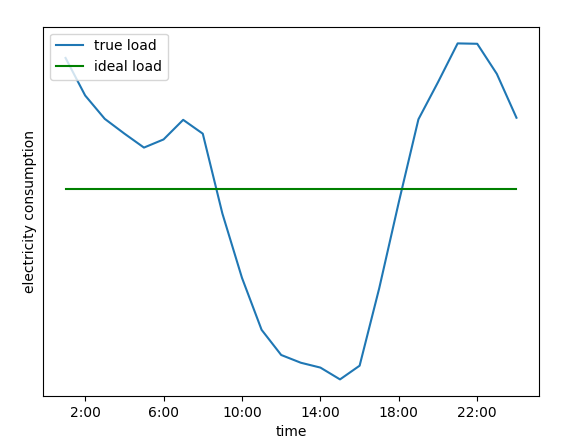
\includegraphics[scale=.75]{figs/duckcurve.png}
    \caption{real power load and the ideal power load for the 
    power grid infrastructure}
    \label{duckcurve}
\end{figure}

Problematic is if a false pricing rumor spreads through social media.
In 2022, changes in the verification policies of Twitter lead to users being able 
to impersonate well-known brands such as Pepsi, leading to Twitter 
users being unable to determine which social media channels were
posting trustworthy information \cite{twitterchaos}. One user could
have used the policy changes of Twitter to impersonate energy companies
and to advertise a false reduction of energy prices, leading to customers
believing the information and increasing their energy consumption as a 
reaction. Another possibility would be that hackers would force access to the
social media profiles of energy companies and start sending false 
information to its customers. Hackers were already able to gain access
to the social media profiles of multinational companies in the past
\cite{twitterhacker}. Hackers could also spread misinformation in regards
to a false reduction in prices, thus leading to changing consumer demand.



% say what demand response is
% then say: yeah its cool for smart homes who can shedule stuff flexibely
% but until then, humans neeed to schedule stuff

\section{Scenario 2: Coordinated Action of Conspiracy Theorists 
against the Electrical Grid}

\section{Scenario 3: Mass Leaving of the City based on Terrorist Attack}

\section{Scenario 4: Mass Showering based on Chemical Accident}
%This Scenario should also be the one with the total framework


% Questions: how to define the parameters
% For some, I can use a dataset and use this as an analogy
% But e.g. scenario 2 it doesnt work well
% how can I put thing out of my ass
% what could be interesting parameter tweakings 